% !TEX root = ../main.tex

\section{The Derivative of a Function}
\begin{theorem}[Derivative]
    The derivative of $f$ is the function
    \begin{equation}
        f'(x) = \lim_{h \to 0}\left(\dfrac{f\left(x + h\right) - f(x)}{h}\right)
    \end{equation}
\end{theorem}
\begin{remark}
    This is only true if the limit exists.
\end{remark}
\begin{corollary}
    If the limit does exist at $x=c$ then $f$ is differentiable at $c$
\end{corollary}
\begin{corollary}
    If the limit exists at every point in interval $\left[a, b\right]$ then $f$ is differentiable on $\left[a, b\right]$. \\
    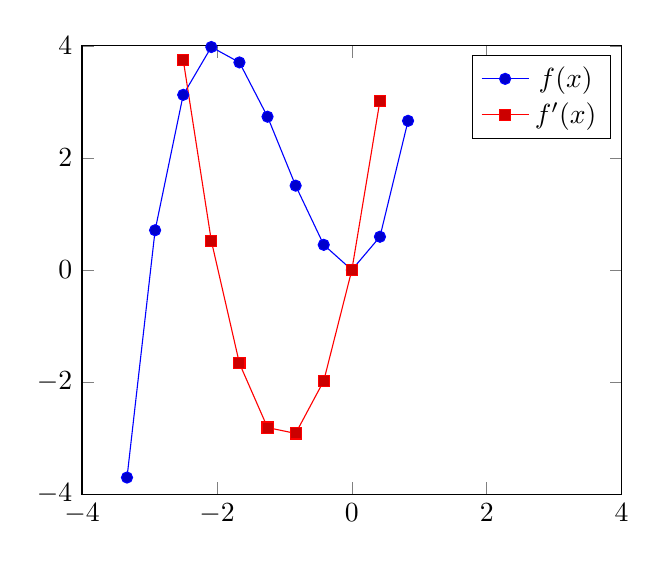
\begin{tikzpicture}
    \begin{axis}[xmin=-4, xmax=4, ymin=-4, ymax=4, restrict y to domain=-4:4]
        \addplot+ {x^3 + 3 * x^2};
        \addplot+ {3 * x^2 + 6 * x};
        \legend{$f(x)$, $f'(x)$};
    \end{axis}
    \end{tikzpicture}
\end{corollary}
\begin{example}
    If $f(x) = x^2 + 2x + 1$ find $f'(x)$.
    \begin{align*}
        f'(x) &= \lim_{h \to 0}\left(\dfrac{f\left(x + h\right) - f(x)}{h}\right) \\
        f'(x) &= \lim_{h \to 0}\left(\dfrac{\left(\left(x+h\right)^2 + 2\left(x + h\right) +1 \right) - \left(x^2 + 2x + 1\right)}{h}\right)\\
        f'(x) &= \lim_{h \to 0}\left(\dfrac{\cancel{x^2} + 2xh + h^2 + \cancel{2x} + 2h + \cancel{1} - \cancel{x^2} - \cancel{2x} - \cancel{1}}{h} \right) \\
        f'(x) &= \lim_{h \to 0}\left( \dfrac{2xh + h^2 + 2h}{h} \right) \\
        f'(x) &= \lim_{h \to 0}\left( 2x + h + 2 \right) \\
        f'(x) &= 2x + 2
    \end{align*}
\end{example}
\begin{example}
    Let $f(x) = \sqrt{x}$. Find $f'(x)$.
    \begin{align*}
        f'(x) &= \lim_{h \to 0}\left( \dfrac{f\left(x + h\right) - f(x)}{h} \right) \\
        f'(x) &= \lim_{h \to 0}\left( \dfrac{\sqrt{x + h} - \sqrt{x}}{h} \right)\\
        f'(x) &= \lim_{h \to 0}\left( \dfrac{\sqrt{x + h} - \sqrt{x}}{h} \cdot \dfrac{\sqrt{x+h} + \sqrt{x}}{\sqrt{x+h} + \sqrt{x}} \right)\\
        f'(x) &= \lim_{h \to 0}\left( \dfrac{\cancel{x} + h - \cancel{x}}{h \left(\sqrt{x + h} + \sqrt{x}\right)} \right)\\
        f'(x) &= \lim_{h \to 0}\left( \dfrac{\cancel{h}}{\cancel{h} \left(\sqrt{x + h} + \sqrt{x}\right)} \right)\\
        f'(x) &= \lim_{h \to 0}\left( \dfrac{1}{\sqrt{x + h} + \sqrt{x}} \right)\\
        f'(x) &= \dfrac{1}{\sqrt{x + 0} + \sqrt{x}}\\
        f'(x) &= \dfrac{1}{2\sqrt{x}}\\
    \end{align*}
\end{example}
\begin{corollary}
    Functions will fail to be differentiable at
    \begin{itemize}
        \item Cusps
        \item Corners
        \item Vertical Tangents
        \item Any point where it is discontinuous
    \end{itemize}
\end{corollary}
\begin{lemma}
    If $f$ is differentiable at $x=c$ then $f$ is continuous at $c$. However a function can be continuous but not differentiable (e.g. $y=\left|x\right|$ at $x=0$).
\end{lemma}
